\newpage
\partie{2}
\section{Insertion}
\begin{prettyBox}{Problem}{myblue}
Il ya des erreurs d'enfrain de l'integrite de la contrainte 
\textcolor{blue}{FOREIGN KEY}
\end{prettyBox}

\vspace{0.25cm}
\textbf{\underline{Code}}
\lstinputlisting{Parties/Partie2/q8.sql}


\vspace{0.25cm}
\textbf{\underline{Output}}

\vspace{0.25cm}
\begin{center}
    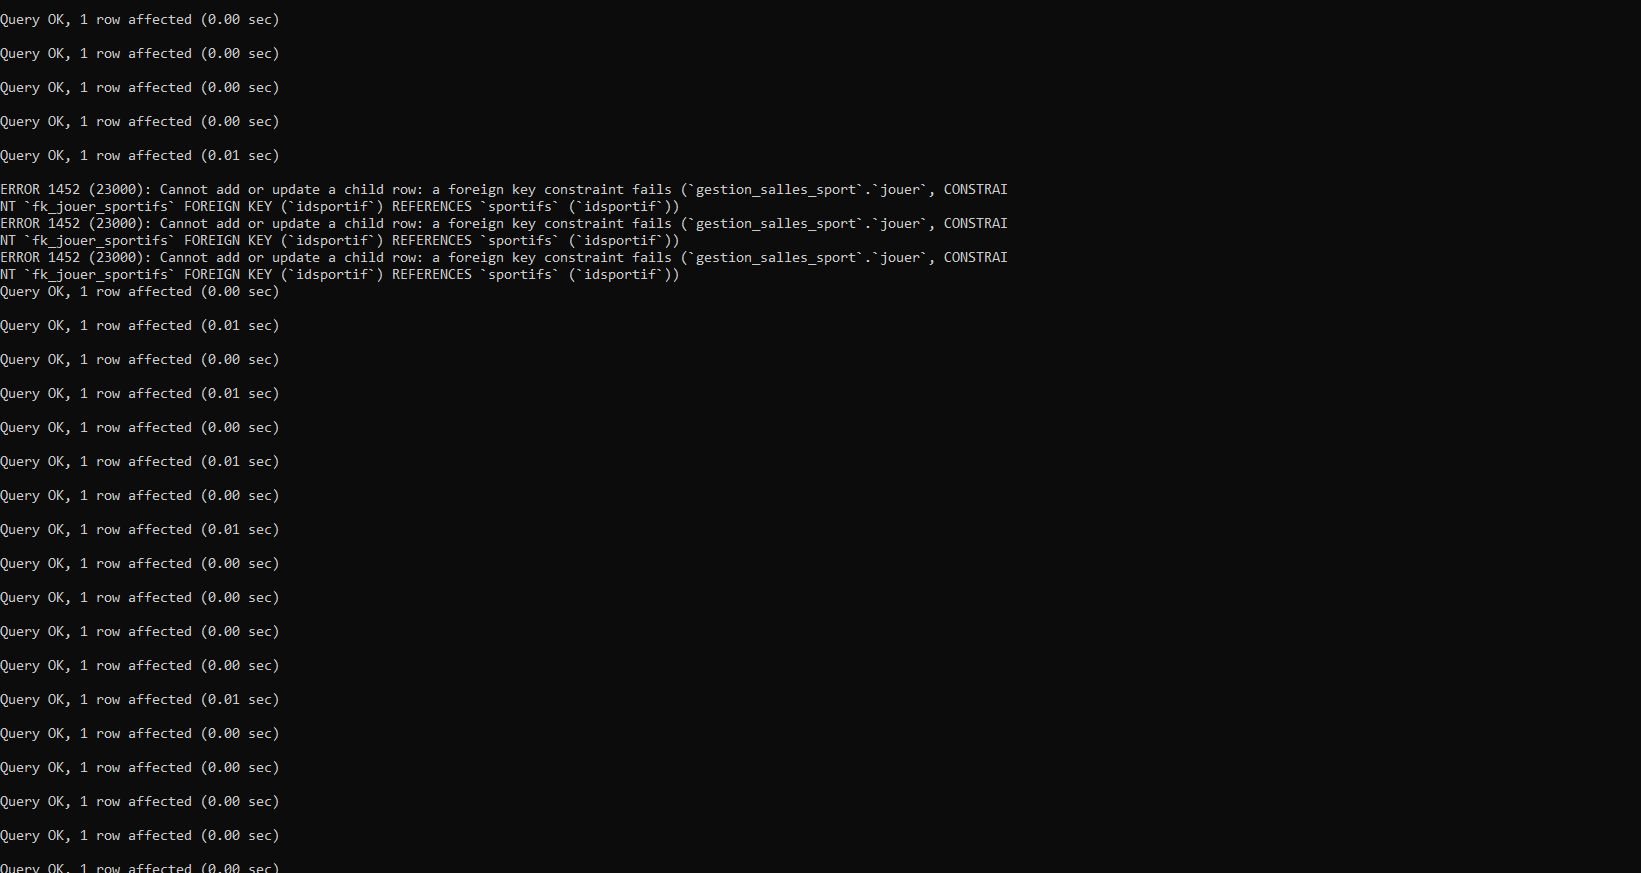
\includegraphics[width=0.8\textwidth]{Parties/Partie2/insert.PNG}
\end{center}

\newpage
\section{Changement De Conseille}
\begin{prettyBox}{Update}{myblue}
    Il est evident qu'on doit faire un \textcolor{blue}{UPDATE} sur la table \texttt{Sportifs} pour 
le sportif \texttt{LACHEMI Bouzid} pour lui change de conseille , mais d'abord
on a besoin de trouver L'\texttt{IdSportif} du nouveau Conseille \texttt{CHAADI Mourad} en 
utilisant un \textcolor{blue}{SELECT} et en stockant la valeur dans une variable qui 
va etre utilise dans l'\textcolor{blue}{UPDATE}.
\end{prettyBox}
\vspace{0.25cm}

\textbf{\underline{Code}}
\lstinputlisting{Parties/Partie2/q9.sql}

\vspace{0.25cm}
\textbf{\underline{Output}}

\vspace{0.25cm}
\begin{center}
    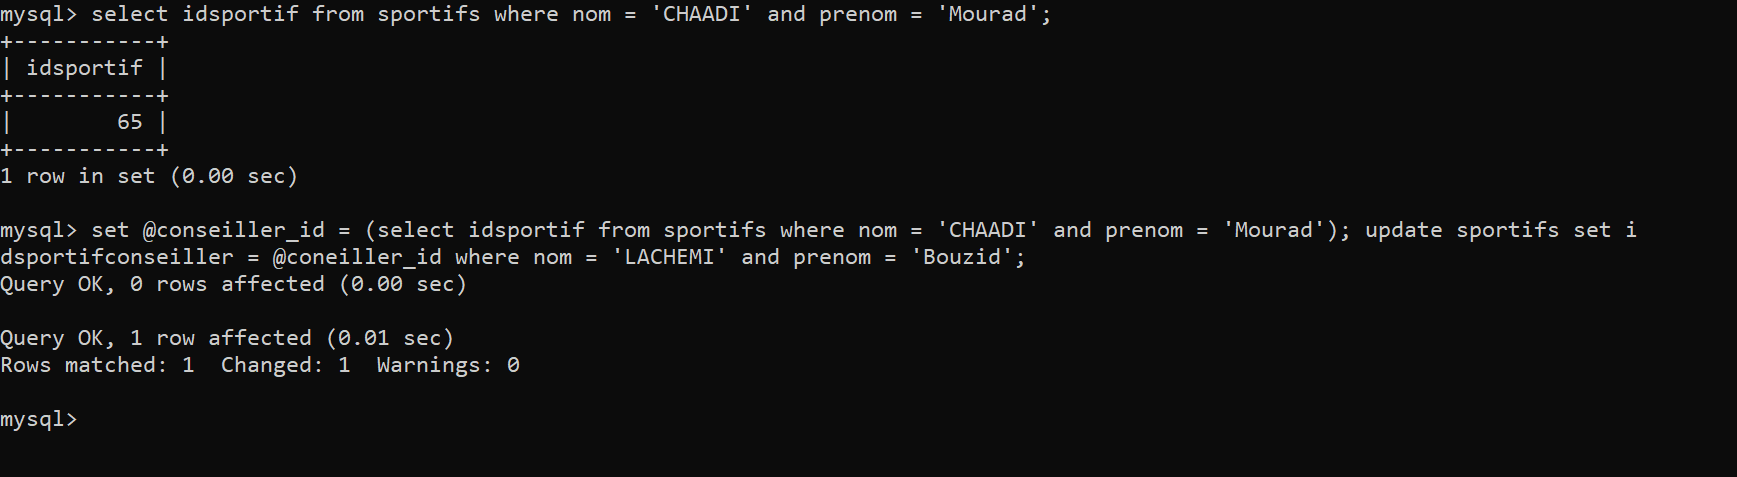
\includegraphics[height=0.25\textheight]{Parties/Partie2/update.PNG}
\end{center}

\newpage
\section{Ajout Des Deux Sport 'Natation' Et 'Golf'}
\begin{prettyBox}{Ajout}{myblue}
On ne peut pas directement inserer les sports 'Natation' et 'Golf' car 
ils ne respectent pas la contrainte \texttt{chk\_sports\_libelle} , de plus
dans \textbf{MySQL} on ne peut pas temporairment desactiver une contrainte 
avec \textcolor{blue}{DISABLE} , donc on doit supprimer la contrainte inserer et la creer a nouveau
avec un check qui accepte 'Natation' et 'Golf'.
\end{prettyBox}

\vspace{0.5cm}
\textbf{\underline{Code}}
\lstinputlisting{Parties/Partie2/q10.sql}

\vspace{1cm}
\section{Supression Des Gymnases}
\begin{prettyBox}{Problem}{myblue}
Si on essaye de supprimer n'importe quelle ligne de la table \texttt{Gymnases} , 
on aura une erreur de contrainte de la cle etrangere puisqu'elle est referance dans
la table \texttt{Seances} , si on voulais regle le problem il foudrait modifier la contrainte
\textcolor{blue}{FOREIGN KEY} en lui ajouttant \textcolor{blue}{DELETE ON CASCADE}
\end{prettyBox}

\vspace{0.5cm}
\textbf{\underline{Code}}
\lstinputlisting{Parties/Partie2/q11.sql}

\vspace{0.5cm}
\textbf{\underline{Output}}
\vspace{0.25cm}
\begin{center}
    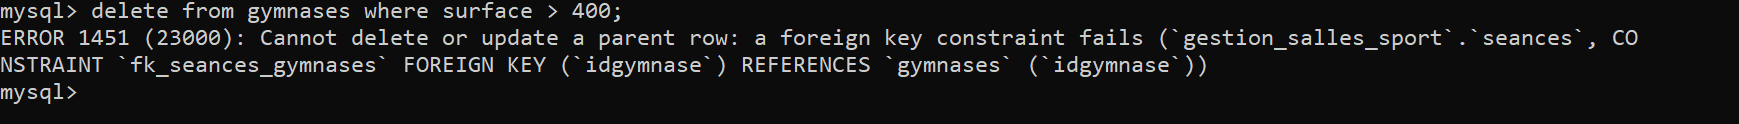
\includegraphics[width=\textwidth]{Parties/Partie2/delete.PNG}
\end{center}



